% Use only LaTeX2e, calling the article.cls class and 12-point type.

\documentclass[12pt]{article}

% Users of the {thebibliography} environment or BibTeX should use the
% scicite.sty package, downloadable from *Science* at
% http://www.sciencemag.org/authors/preparing-manuscripts-using-latex 
% This package should properly format in-text
% reference calls and reference-list numbers.

\usepackage{scicite}
\usepackage{hyperref}
\providecommand{\tightlist}{%
  \setlength{\itemsep}{0pt}\setlength{\parskip}{0pt}}

\usepackage{times}
\usepackage{graphicx}
\usepackage{float}

% The preamble here sets up a lot of new/revised commands and
% environments.  It's annoying, but please do *not* try to strip these
% out into a separate .sty file (which could lead to the loss of some
% information when we convert the file to other formats).  Instead, keep
% them in the preamble of your main LaTeX source file.


% The following parameters seem to provide a reasonable page setup.

\topmargin 0.0cm
\oddsidemargin 0.2cm
\textwidth 16cm 
\textheight 21cm
\footskip 1.0cm


%The next command sets up an environment for the abstract to your paper.

\newenvironment{sciabstract}{%
\begin{quote} \bf}
{\end{quote}}



% Include your paper's title here

\title{Documentation and reproducibility with R and \LaTeX\ } 


% Place the author information here.  Please hand-code the contact
% information and notecalls; do *not* use \footnote commands.  Let the
% author contact information appear immediately below the author names
% as shown.  We would also prefer that you don't change the type-size
% settings shown here.

\author
{Monikrishna Roy,$^{1\ast}$ Perry J. Williams,$^{2}$\\
\\
\normalsize{$^{1}$Department of Computer Science and Engineering, University of Nevada, Reno}\\
\normalsize{$^{2}$Department of Natural Resources and Environmental Science, University of Nevada, Reno}\\
\\
\normalsize{$^\ast$To whom correspondence should be addressed; E-mail:  monikrishna@nevada.unr.edu.}
}

% Include the date command, but leave its argument blank.

\date{}



%%%%%%%%%%%%%%%%% END OF PREAMBLE %%%%%%%%%%%%%%%%



\begin{document}

% Double-space the manuscript.

\baselineskip24pt

% Make the title.

\maketitle



% Place your abstract within the special {sciabstract} environment.

\begin{sciabstract}
      The reproducible research workshop covers basic usage of R, RStudio, Latex, and knitr to develop a workflow for research documentation and reproduction. The reproducible research workshop was developed from the book Reproducible Research with R and RStudio, by Christopher Gandrud \cite{glennie2021reproducible}.
\end{sciabstract}



% In setting up this template for *Science* papers, we've used both
% the \section* command and the \paragraph* command for topical
% divisions.  Which you use will of course depend on the type of paper
% you're writing.  Review Articles tend to have displayed headings, for
% which \section* is more appropriate; Research Articles, when they have
% formal topical divisions at all, tend to signal them with bold text
% that runs into the paragraph, for which \paragraph* is the right
% choice.  Either way, use the asterisk (*) modifier, as shown, to
% suppress numbering.

\section*{Introduction}

GRAD 778 introduces broadly applicable skills relevant for understanding the rapidly changing technological landscape of the 21 st century. Further, skills developed in this course are directly supportive to Reno’s research technology economy. This course builds human capital with research computing skills that are timely and necessary for current, local employment. Computational research is essential to understanding the complexities facing the modern workforce, and graduates of GRAD 788 will be required to handle sample datasets and learn to navigate and choose amongst various research computing skill sets.

This course is an overview of computational research as well as a skills-based introduction to programming and shell scripting for automating computational tasks. This course is offered for variable credit depending on the number of weekend workshops a student selects at the start of the semester.

Anyone interested in using computational tools for research in any graduate department is encouraged to attend. Students will have the opportunity to work hands-on with large datasets with various real-world examples and write basic programs in more than one programming language. Classes will be part lecture, part open discussion, and part hands-on practice, held in mini-session format and lessons will be fully inclusive within each workshop.

Class materials in a mini-workshop format will be posted online in video format, and then discussion sessions held live on Saturdays. Students will select from the mini-workshops of interest. Mandatory attendance is required at course introduction during the first week (August 29 th ) of classes to establish proper equipment and enrollment.

To receive one graduate credit, a minimum of three-weekend workshops must be attended in full. To receive two graduate credits, a minimum of six-weekend workshops must be attended in full. To receive three graduate credits, a minimum of nine-weekend workshops must be attended in full. To receive course credit, students must display a working piece of code and pass a quiz at the end of each workshop.

``Documentation and reproducibility with R and \LaTeX\ " is a workshop of GRAD 778 courses.

\section{Course Overview}

\subsection{Video Lectures}

\begin{itemize}
      \tightlist
      \item
            \href{https://youtu.be/5isfqu7dhmk}{Introduction}
      \item
            \href{https://youtu.be/qk4YiRPovNM}{Installation}
      \item
            \href{https://youtu.be/Ec3jqBKuXyk}{LaTeX}
      \item
            \href{https://youtu.be/LGOApODWJlE}{knitR}
      \item
            \href{https://youtu.be/C1Xv3riRZno}{Conclusion}
\end{itemize}


\subsection{Overview of Files}

\hypertarget{rep-res-workshop}{%
      \subsubsection{Rep-Res-Workshop}\label{rep-res-workshop}}

The parent directory for the workshop is a file called Rep-Res-Workshop. Within this file are three files, including Analysis, Data, and Presentation.

\hypertarget{analysis}{%
      \paragraph{Analysis}\label{analysis}}

The analysis file contains an R script file called \textbf{MainAnalysis.R} that was used to analyze avian species richness in the United States. It also contains a sub-file called ResultsFigures, which includes .pdf output of figures from the \textbf{MainAnalysis.R} file.

\hypertarget{data}{%
      \paragraph{Data}\label{data}}
The data file contains the avian species richness \textbf{data.csv} file used in
the \textbf{MainAnalysis.R} script.

\hypertarget{presentation}{%
      \paragraph{Presentation}\label{presentation}}

The presentation file contains seven sub-files. Four files contain examples used during the workshop. Two files contain exercises used during the workshop. One file contains the documents required to compile the workshop lecture pdf.

\section{Materials}

\hypertarget{installing-the-main-software-for-the-workshop}{%
      \subsection{Installing the Main Software for the
            Workshop}\label{installing-the-main-software-for-the-workshop}}

Before coming to the workshop you should install the main software. All of the software programs covered in the workshop are open source and can be easily downloaded for free. They are available for Windows, Mac, and
Linux operating systems. They should run well on most modern computers.

You should install R before installing RStudio. You can download the programs from the following websites:

\begin{itemize}
      \tightlist
      \item
            \href{http://www.r-project.org/}{R}\cite{citeR}
      \item
            \href{http://www.rstudio.com/ide/download}{RStudio}\cite{citeRStudio}
\end{itemize}

The download webpages for these programs have comprehensive information on how to install them, so please refer to those pages for more
information. After installing R and RStudio you will want to install a number of user-written packages that are covered in this workshop. To install all of these user-written packages, run the following command in
R:

\begin{verbatim}
required.packages=c("formatR","here","knitr","Matrix")
lapply(required.packages,install.packages,character.only=TRUE)
lapply(required.packages,library,character.only=TRUE)
\end{verbatim}

\hypertarget{installing-markup-language}{%
      \subsection{Installing markup
            language}\label{installing-markup-language}}

To create \LaTeX\ documents you need to install a \TeX\ distribution. They are
available for Windows, Mac, and Linux systems. They can be found at:
\url{http://www.latex-project.org/ftp.html}. Please refer to that site
for more installation information.

\hypertarget{session-info}{%
      \subsection{Session Info}\label{session-info}}

\begin{verbatim}
toLatex(sessionInfo())
\end{verbatim}

\begin{itemize}
      \item
            R version 3.6.0 (2019-04-26),x86\_64-apple-darwin15.6.
      \item
            Locale:
            en\_US.UTF-8/en\_US.UTF-8/en\_US.UTF-8/C/en\_US.UTF-8/en\_US.UTF-
      \item
            Running under:macOS Mojave 10.14.
      \item
            Matrix products: default
      \item
            BLAS:
            /Library/Frameworks/R.framework/Versions/3.6/Resources/lib/libRblas.0.dylib
      \item
            LAPACK:
            /Library/Frameworks/R.framework/Versions/3.6/Resources/lib/libRlapack.dylib
      \item
            Base packages: base, datasets, graphics, grDevices, methods, stats,
            utils
      \item
            Other packages: formatR 1.7, here 0.1, knitr 1.25, Matrix 1.2-
      \item
            Loaded via a namespace (and not attached): backports 1.1.4, compiler
            3.6.0, evaluate 0.14, grid 3.6.0, highr 0.8, lattice 0.20-38, magrittr
            1.5, rprojroot 1.3-2, stringi 1.4.3, stringr 1.4.0, tcltk 3.6.0, tools
            3.6.0, xfun 0.
\end{itemize}

\section{Example of Tables and Figures}

Following are a few example handling the table and figures.

\paragraph*{Tables.}  The Table \ref{table:1} is showing head the data provided in the workshop directory.

\begin{table}[h!]
      \centering
      \begin{tabular}{||c c c c c c c c||}
            \hline
            rank & state      & st & spp & area    & temp & precip & statename  \\ [0.5ex]
            \hline\hline
            17   & Alabama    & AL & 326 & 135765  & 62.8 & 58.3   & alabama    \\
            46   & Alaska     & AK & 269 & 1717854 & 26.6 & 22.5   & alaska     \\
            3    & Arizona    & AZ & 435 & 295254  & 60.3 & 13.6   & arizona    \\
            22   & Arkansas   & AR & 312 & 137732  & 60.4 & 50.6   & arkansas   \\
            4    & California & CA & 415 & 423970  & 59.4 & 22.2   & california \\
            \hline
      \end{tabular}
      \caption{Head of the dataset provided in the workshop.}
      \label{table:1}
\end{table}

\paragraph*{Figures.}  Figures \ref{fig:finaldoc} \& \ref{fig:gitcomments} are taken from the example figure of the workshop.

\begin{figure}[H]
      \centering
      \begin{minipage}[b]{0.4\textwidth}
            
\includegraphics[width=\textwidth]{figs/finaldoc.png}
            \caption{Final Doc Picture}
            \label{fig:finaldoc}
      \end{minipage}
      \hfill
      \begin{minipage}[b]{0.5\textwidth}
            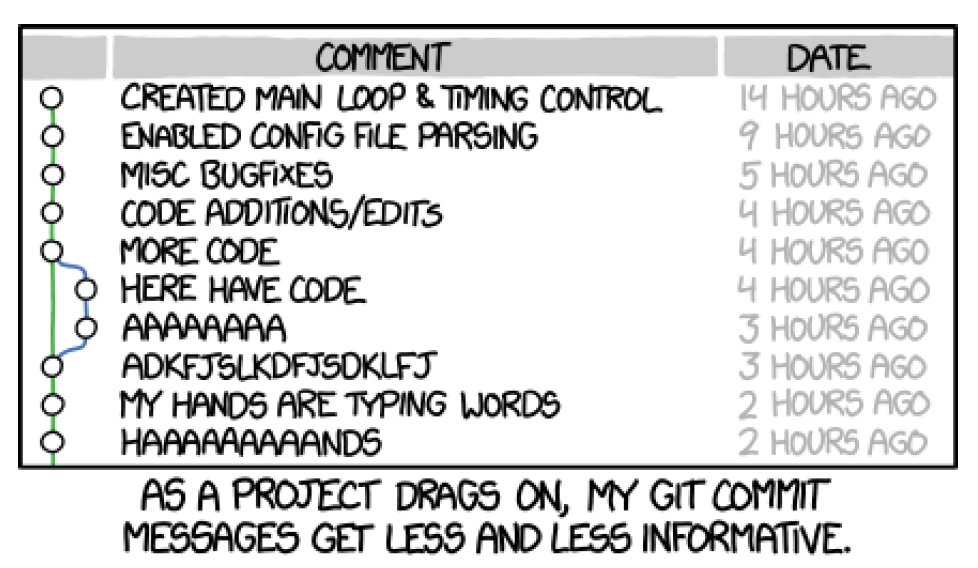
\includegraphics[width=\textwidth, height=8cm]{figs/gitcomments.png}
            \caption{Git Comments Example}
            \label{fig:gitcomments}
      \end{minipage}
\end{figure}

\section{Conclusion}
The purpose of the workshop is developing a workflow to maximize reproducible research and research impact in computational science: managing data, computer code, and analyses output. Examples will include combining LaTeX, R, and knitR\cite{citeKnitr}.
% Your references go at the end of the main text, and before the
% figures.  For this document we've used BibTeX, the .bib file
% scibib.bib, and the .bst file Science.bst.  The package scicite.sty
% was included to format the reference numbers according to *Science*
% style.

%BibTeX users: After compilation, comment out the following two lines and paste in
% the generated .bbl file. 

\bibliography{scibib}

\bibliographystyle{Science}


\section*{Acknowledgments}
Thanks to the instructor for the wonderful workshop.

%Here you should list the contents of your Supplementary Materials -- below is an example. 
%You should include a list of Supplementary figures, Tables, and any references that appear only in the SM. 
%Note that the reference numbering continues from the main text to the SM.
% In the example below, Refs. 4-10 were cited only in the SM.     
\section*{Supplementary materials}
All code and lecture sheets will be found in the Canvas.


% For your review copy (i.e., the file you initially send in for
% evaluation), you can use the {figure} environment and the
% \includegraphics command to stream your figures into the text, placing
% all figures at the end.  For the final, revised manuscript for
% acceptance and production, however, PostScript or other graphics
% should not be streamed into your complied file.  Instead, set
% captions as simple paragraphs (with a \noindent tag), setting them
% off from the rest of the text with a \clearpage as shown  below, and
% submit figures as separate files according to the Art Department's
% instructions.
\end{document}




















